\chapter{Design and Implementation}


The main goal of this thesis is to be able to recognize asbestos fibers in microscopic images. To achieve that goal different CNN architectures are evaluated and altered to better meet this specific problems' characteristics. Different methods like transfer learning and data augmentation are applied to this problem in hope to further increase the accuracy. This is especially important, since the provided dataset consists of only a few hundred images to learn from. There is no baseline available, so a new baseline needs to be established with a simple CNN.

\section{Problem Description}

The provided dataset consists of about 2'000 microscopic images with and without asbestos fibers. The images come in two different dimensions and different qualities. Most of the images are 1024 by 768 pixels but some are in 1024 by 1024 pixels. Only a small subset was pre-labled and the remaining images needed to be labeled by hand, an error-prone task since I was never professionally instructed on how to do it. After labeling the images, they were send back to the laboratories for checking, but there were many images, that the experts were uncertain on how to label them. From 441 images I labeled and send the laboratory for checking 78 images came back as being suspected to contain asbestos but they were not quite sure. That's about 5.65\%. The detection of traces of asbestos by images is indeed very difficult and the error rate increases significantly as stated by the laboratory. In Figure \ref{fig:basic_examples} three example images are shown. One with asbestos, one without and one image with an error, that makes it difficult to be used for the training.

\begin{figure}[t]
\centering
\subfigure[Example with an asbestos fiber spanning from top to down]{
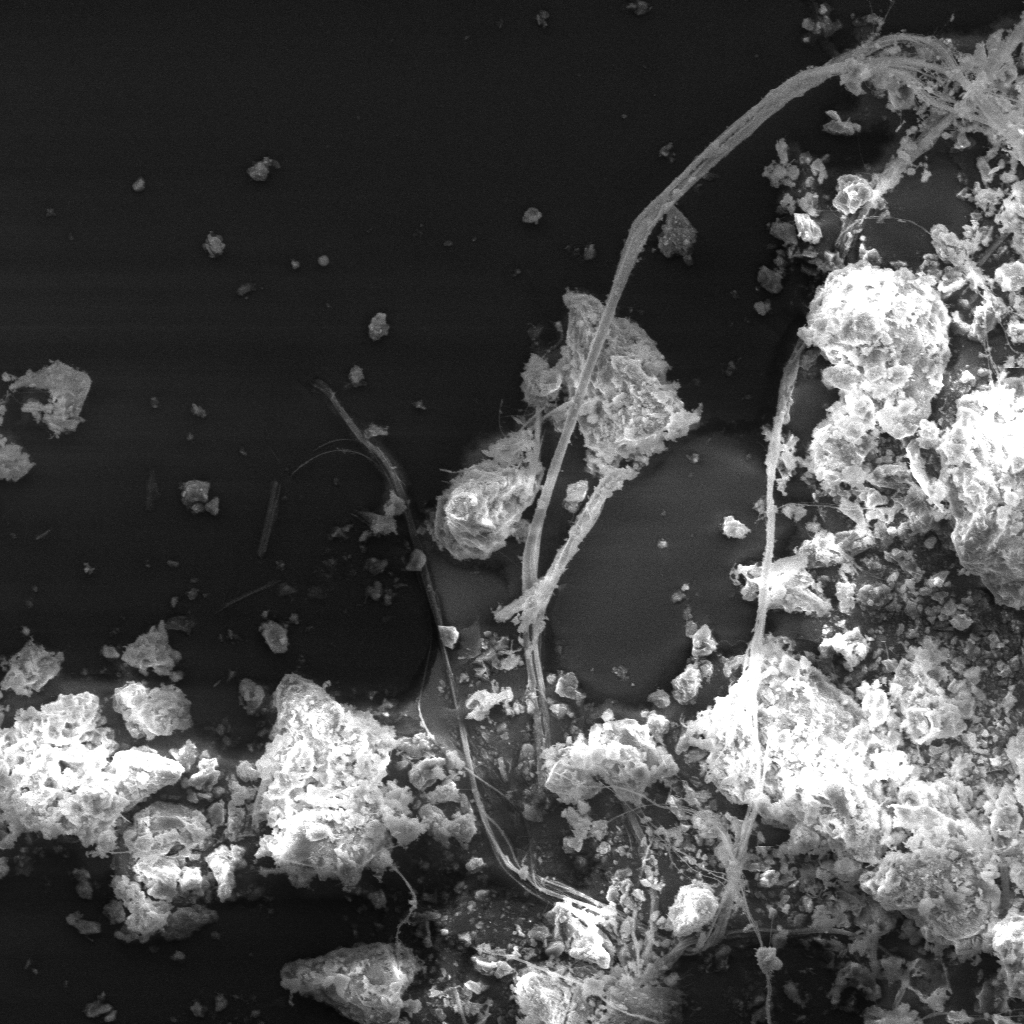
\includegraphics[width=.3\textwidth]{images/chapter5/asbestos.png}
}
\subfigure[Example without any asbestos fibers]{
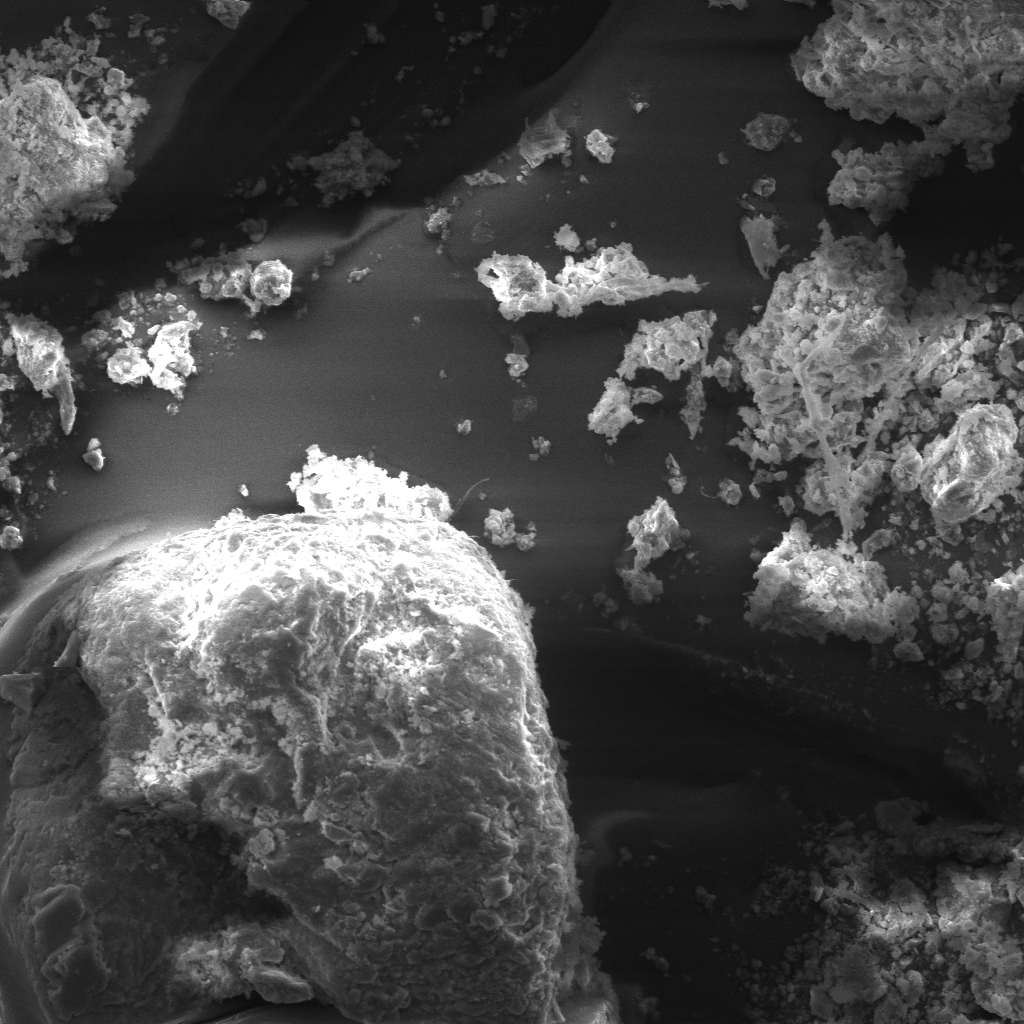
\includegraphics[width=.3\textwidth]{images/chapter5/non-asbestos.png}
}
\subfigure[Example of one kind of error, that makes the image unusable]{
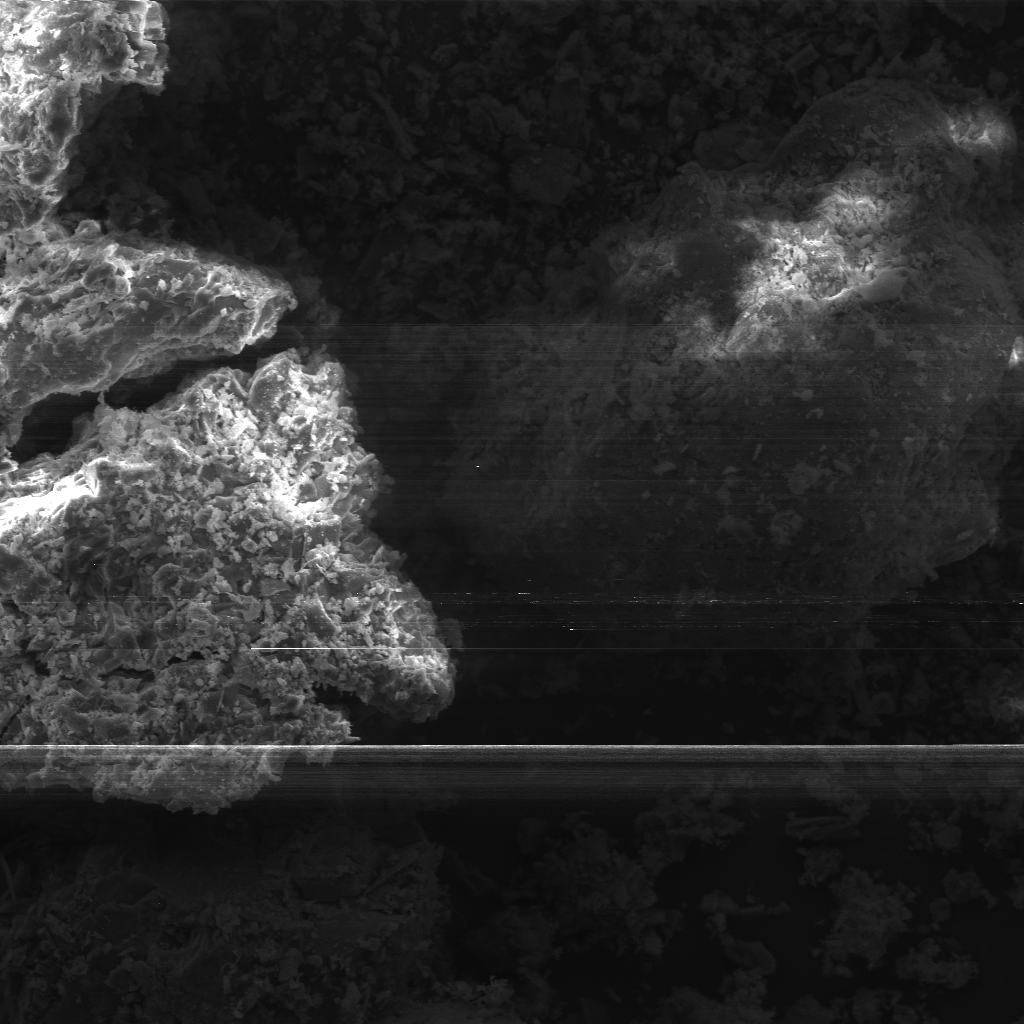
\includegraphics[width=.3\textwidth]{images/chapter5/fail.png}
}


\caption{Some examples on how the microscopic images look like, and what kind of error in images occur.}
\label{fig:basic_examples}
\end{figure}

Since the images are quite large, they will drastically increase in size, once decoded into a PIL object, or Tensor object. Therefore it will be difficult to train on the whole image due to GPU resource restrictions. For the project, four Tesla K80 with 12GB of RAM each were provided.

[**I think the 0.1\% they mention holds true only for clear cases where there is lots of asbestos.**]

\section{Data Augmentation}

There are only a few hundred good and usable images provided for the asbestos recognition task. Additionally they are highly specialized in how they were done. With specific cameras and in specific environments in a specific zoom. Finding more images on the internet is impossible so data augmentation could possibly lead to an increased dataset with more images to train on and therefore increase performance. A huge dataset is required to be able to generalize the model and to perform well on a test set. Transfer learning might help but the fine tuning needs to be done after transferring the weights to the current task.

There 

\section{AlexNext}

It has not been possible to get a baseline for the current performance or even an accurate estimation of human performance in the detection of asbestos fibers in the provided images. Therefore, AlexNet was used to create a baseline on which improvements may be observed and would allow discussions on architectures and their performance. The hyper-parameters learning rate and learning rate decay have been optimized with grid search by running every configuration five times, averaging the results and choosing the hyper-parameters that performed best.

\begin{table}[t] \centering
\ra{1.3}
\caption{AlexNet accuracies for baseline with optimized hyper-parameters}
\begin{tabular}{@{}rrrr@{}}
\toprule & learning rate & lr-decay & accuracy \\
\midrule
AlexNet		& 0.1 		& 5		& 52.18\%  \\
AlexNet		& 0.05 		& 5		& 53.64\%  \\
AlexNet		& 0.01 		& 5		& 53.37\%  \\
AlexNet		& 0.005 		& 5		& 53.67\%  \\
AlexNet		& 0.001 		& 5		& 78.82\%  \\
AlexNet		& 0.0005 		& 5		& 78.55\%  \\
AlexNet		& 0.0001 		& 5		& 77.09\%  \\
\bottomrule
\end{tabular}
\label{tbl:similarity-test-map}
\end{table}


\section{Inception / ResNet}

Talk about other architectures and why they are important

\section{SigOpt Optimization}

What is SigOpt and why did I use it?
